\documentclass{article}
\usepackage[italian]{babel}
\usepackage[T1]{fontenc}
\usepackage{graphicx}
\usepackage[utf8x]{inputenc}
\usepackage{amsmath}
\usepackage{amsthm}
\usepackage{hyperref}
\date{Novembre 2015}
\author{Francesco Sacco, Lorenzo Cavuoti}
\title{Usi non lineari dell'OpAmp}

\begin{document}
	\maketitle
	\section{Amplificatore di carica}
		Per spiegare il circuito dell'amplificatore di carica è meglio analizzarlo con i suoi due sotto-circuiti separatamente, e poi vedere come si incastrano assieme.\newline
		\subsection{Teoria Primo sotto-circuito}
			Il primo sottocircuito è quello che è collegato al voltaggio in ingresso $V_S$, esso si può vedere nella figura \ref{fig:circ1}
			\begin{figure}
				\label{fig:circ1}
				\centering
				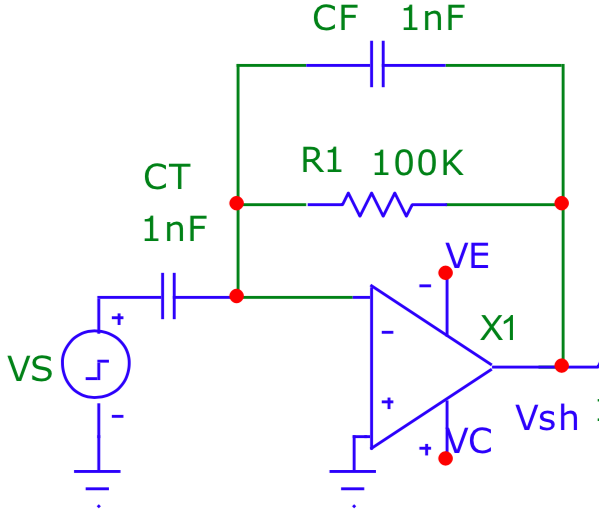
\includegraphics[width=70mm]{immagini/circ1b.png}
				\caption{sotto-circuito 1}
			\end{figure}
			, risolvere il circuito equivale a risolvere questo sistema di 3 equazioni
			\begin{equation}
				\begin{cases}
					V_s-V_-=\frac{Q_T}{C_T}\\
					V_--V_{sh}=I_1R_1\\
					V_--V_{sh}=\frac{Q_F}{C_F}
				\end{cases}
			\end{equation}
			Derivando rispetto al tempo la prima e la terza equazione, supponendo che $\frac{dV_s}{dt}=0$\footnote{visto che è un'onda quadra possiamo supporre di interessarci al circuito nei punti in cui l'onda quadra è costante}, e imponendo che $V_{sh}=AV_-$ si ottiene
			\[
				\begin{cases}
					\frac{dV_-}{dt}=-\frac{I_T}{C_T}\\
					(1+A)V_-=I_1R_1\\
					(1+A)\frac{dV_-}{dt}=\frac{I_F}{C_F}
				\end{cases}
				\begin{cases}
					\frac{dV_-}{dt}=-\frac{I_1+I_F}{C_T}\\
					I_F=C_F(1+A)\frac{dV_-}{dt}\\
					I_1=\frac{1+A}{R_1}V_-
				\end{cases}
			\]
			Passando dal primo sistema all'altro ho usato che $I_T=I_1+I_F$, sostituendo $I_1$ e $I_F$ nella prima equazione si ottiene che
			\[
				\frac{dV_-}{dt}=\frac{1}{C_T}\bigg[C_F(1+A)\frac{dV_-}{dt}+\frac{1+A}{R_1}V_-\bigg]
			\]
			\[
				\frac{dV_-}{dt}\bigg[\frac{C_T}{1+A}+C_F\bigg]=-\frac{V_-}{R_1}
			\]
			Nel limite in cui $A$ è molto grande possiamo considerare $\frac{C_T}{1+A}\approx0$, quindi l'equazione di prima diventa
			\[
				\frac{dV_-}{dt}\approx-\frac{V_-}{C_FR_1}\qquad\qquad
				A\frac{dV_-}{dt}\approx-A\frac{V_-}{C_FR_1}\qquad\qquad
				\frac{dV_{sh}}{dt}\approx-\frac{V_{sh}}{C_FR_1}
			\]
			Quindi si ottiene dal primo sottocircuito che\newline
			\begin{equation}
				V_{sh}=V_0e^{-t/C_FR_1}
			\end{equation}
			CONTROLLA SE $V_0$ E' UGUALE A $V_S$!!!
		\subsection{Teoria secondo sotto-circuito}
			Prima di spiegare direttamente il secondo sottocircuito è meglio dare un paio di informazioni parecchio approssimative sull'OpAmp.\newline
			L'OpAmp è un dispositivo a 5 terminali, per indicare il voltaggio in ciascun terminale useremo la convenzione dell'immagine \ref{fig:OpAmp1}\newline
			\begin{figure}
				\label{fig:OpAmp1}
				\centering
				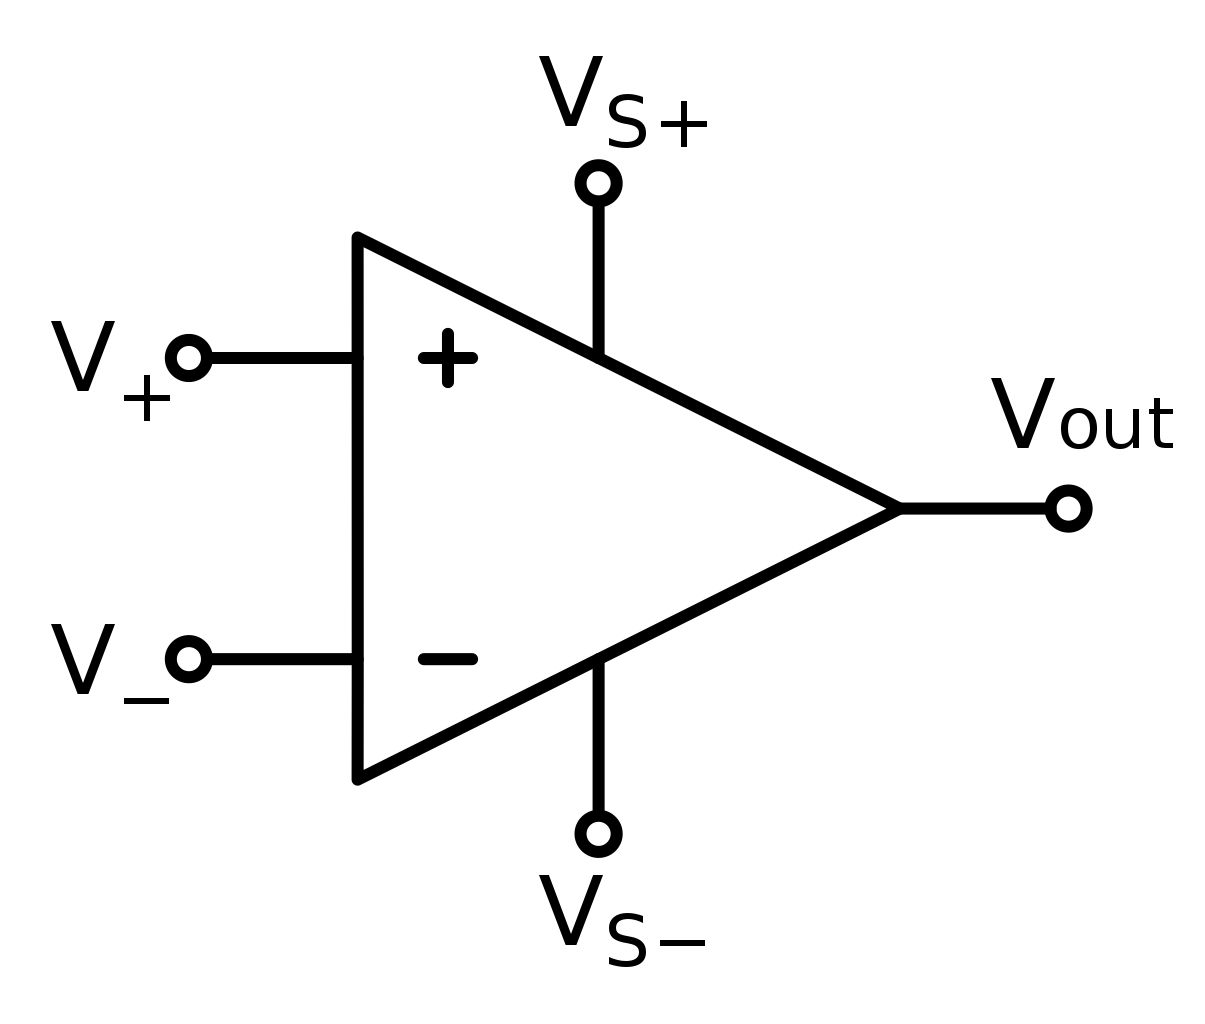
\includegraphics[width=40mm]{immagini/OpAmp1.png}
				\caption{un OpAmp}
			\end{figure}
			L'OpAmp è in grado di amplificare il segnale per bene solo se $V_{S-}<A(V_+-V_-)<V_{S+}$, se per caso $A(V_+-V_-)>V_{S+}$, l'amplificatore porta $V_{out}$ al massimo voltaggio che può dare, cioè $V_{S+}$, e se $A(V_+-V_-)<V_{S-}$ $V_{out}=V_{S-}$.\newline

			Essendo $A$ molto grande basta una differenza di potenziale molto piccola ai capi dei terminali + e - per mandare l'OpAmp a $V_{S+}$ e $V_{S-}$, quindi ciò viene usato per dire in modo binario se un voltaggio è maggiore di un'altro voltaggio, infatti se $A|V_+-V_-|>>1$ si ha che $V_{out}=V_{S+}$ se $V_+>V_-$ e $V_{out}=V_{S-}$ se $V_+<V_-$.\newline

			Adesso che sappiamo ciò possiamo spiegare il secondo sottocircuito:
			Il secondo sotto circuito si può vedere nella figura \ref{fig:circ2}, il terminale positivo è collegato a $V_{sh}$ attraverso una resistenza di $100\Omega$, quindi visto che la corrente che passa per il terminale positivo è circa zero possiamo assumere che la differenza di potenziale ai capi sia trascurabile.\newline
			Chiamerò $V_P$\footnote{P sta per potenziometro} il potenziale che va nel terminale negativo dell'OpAmp, esso è possibile regolarlo grazie all'ausilio del potenziometro che funge da partitore di tenzione.\newline
			Essendo (quasi sempre) $A|V_{sh}-V_P|>>1$ si ha che $V_{discr}=V_C$ se $V_{sh}>V_P$ e che $V_{discr}=V_E$ se $V_{sh}<V_E$.
			\begin{figure}
				\label{fig:circ2}
				\centering
				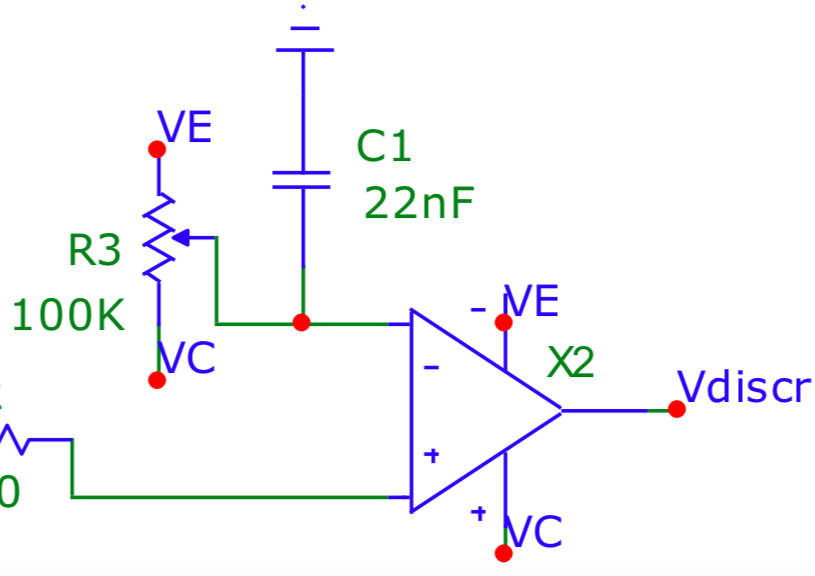
\includegraphics[width=70mm]{immagini/circ2a.png}
				\caption{sotto-circuito 2}
			\end{figure}
		\subsection{Quello che resta della Teoria}
			asd



\end{document}